\documentclass[aps,reprint]{revtex4-2}
\usepackage{listings}
\usepackage{graphicx}
\usepackage{float}
\usepackage{lipsum}
\usepackage[spanish]{babel}
\usepackage{amsmath}
\usepackage{amssymb}



\begin{document}
\title{Análisis del comportamiento lector en México: hallazgos del Módulo sobre Lectura (MOLEC)}\thanks{Liga al repositorio del proyecto: github.com/Lunaaaalj/MEPTD}
\author{Ángel Eduardo Luna Leija\\Rafael Sánchez Ramírez\\Sebastián Cortés Quiroz\\Emilio Alonso Sánchez}
\affiliation{Instituto Tecnológico y de Estudios Superiores de Monterrey}
\date{\today}
\begin{abstract}
El presente estudio analiza la relación entre los estímulos lectores en la infancia y el desarrollo del hábito de lectura en la edad adulta en México, utilizando como fuente de información el Módulo sobre Lectura (MOLEC) del INEGI. A partir de una selección de variables sociodemográficas, experiencias infantiles (bloque P34) y hábitos lectores actuales, se realizó una primera etapa de análisis descriptivo para explorar patrones en los datos. Los resultados preliminares muestran que la mayoría de los adultos mexicanos reportan hábitos lectores bajos en términos de frecuencia e intensidad, con altos niveles de concentración en valores cercanos a cero textos leídos al año. Sin embargo, se observa una asociación consistente entre la presencia de estímulos familiares tempranos —como ver a los padres leer o tener libros en casa— y una mayor propensión a leer por gusto en la adultez. Si bien esta fase descriptiva no permite establecer causalidad, los hallazgos sugieren que el capital cultural del hogar podría tener un peso comparable o incluso superior al de la educación formal en la formación del hábito lector. En la siguiente etapa del proyecto se aplicarán pruebas inferenciales y modelos estadísticos para validar estas relaciones y determinar qué estímulos infantiles tienen mayor impacto en la lectura por placer.
\end{abstract}
\maketitle
\tableofcontents



\section{Etapa: Introducción al Reto}
\subsection{Introduccion}
La medición del estado de la lectura en México es fundamental para comprender cómo se desarrollan los hábitos lectores y, al mismo tiempo, para identificar las desigualdades culturales y educativas que persisten en la sociedad. La lectura no solo es una actividad escolar o académica, sino también una práctica cotidiana que abre puertas al conocimiento, al pensamiento crítico y a la participación social. Por ello, conocer cómo, cuándo y por qué leen las personas en México permite tener un panorama más claro de la realidad cultural del país.\cite{noauthor_modulo_2020}
En un contexto donde el acceso a los libros y la formación de hábitos lectores desde la infancia son elementos clave, la encuesta MOLEC del INEGI se convierte en una herramienta esencial para detectar patrones, reconocer diferencias y señalar áreas de oportunidad. Esta encuesta no se limita únicamente a recopilar cifras, sino que también refleja las condiciones sociales y culturales que influyen en la lectura en diferentes sectores de la población.\cite{noauthor_modulo_2020}
Es importante subrayar que la lectura no se encuentra determinada únicamente por la educación formal. 

El capital cultural adquirido en el hogar juega un papel decisivo en la formación de los hábitos lectores. Investigaciones como las de Hernández\cite{hernandez_impacto_2020} y Garcia\cite{garcia_lectura_nodate} muestran que crecer en un entorno familiar donde se fomenta la lectura desde edades tempranas es un factor que predice con mayor fuerza la continuidad de esta práctica en la edad adulta, aun cuando el nivel educativo formal no sea elevado.
Asimismo, el análisis del estado de la lectura en México enfrenta retos particulares: la amplia diversidad regional, las diferencias socioeconómicas y la desigualdad en la disponibilidad de recursos dentro de los hogares. Estos desafíos también se observan en otros países, lo que ha motivado a organismos internacionales como la UNESCO a señalar la importancia de atender estas brechas para garantizar que el derecho a la lectura sea accesible a todas las personas, independientemente de su contexto social y cultural.\cite{noauthor_informe_2021}

La motivación del INEGI al realizar la encuesta MOLEC radica en obtener información precisa y confiable que permita orientar la creación de políticas públicas dirigidas a fomentar la lectura desde la infancia. De esta manera, se busca no solo promover el hábito lector, sino también reducir las brechas culturales que persisten. Diversos informes señalan que, gracias a este tipo de mediciones, se han logrado avances importantes en la comprensión de los hábitos lectores en México y en la identificación de los principales obstáculos que impiden que más personas se acerquen a la lectura de manera constante.\cite{noauthor_modulo_2020}
% Describe el problema específico que abordarán (preguntas de investigación u objetivo del proyecto)
%Justifica tu pregunta de indagación en términos de por qué es importante indagar en estos temas en términos del impacto social que puede tener. Debes retomar la PARTE I para concretar la importancia de tu pregunta dentro de la problemática general del reto
\subsection{Objetivo de investigacion}
\subsubsection{Planteamiento del problema específico}
La problemática que enfrentamos sobre la lectura en México no solo se presenta en la frecuencia con la que los adultos leen, sino en la raíz que origina ese origen de carencias. Todo viene desde la desigualdad de oportunidades desde la infancia. Existen estudios y datos de la encuesta MOLEC que nos muestran que los hábitos de lectura a temprana edad sí influyen en la disposición y frecuencia de lectura en personas mayores. Pero se debe determinar si el desarrollo del hábito de leer depende principalmente de la educación formal que se recibe en escuelas o está más relacionado con un estándar cultural que se adquiere en el núcleo familiar.  

Es por eso que nuestro proyecto se centra en una problemática más acotada: \textbf{el desarrollo del hábito de la lectura en la edad adulta no está determinado principalmente por la educación formal recibida, sino por el capital cultural adquirido en el hogar durante la infancia}. La presencia de libros y de un entorno familiar lector son los predictores más fuertes de si un mexicano será o no un lector por gusto en su vida. En la hipótesis central se sostiene que los adultos que tuvieron el apoyo a edad temprana, como por ejemplo escuchar a sus padres leer, tener libros en casa o asistir a bibliotecas, muestran una mayor probabilidad de ser lectores por gusto en la actualidad, independientemente de su nivel máximo de estudios.  

Con este planteamiento abordamos una pregunta esencial: \textit{¿Qué tiene mayor peso en el hábito lector de un adulto, la escuela o los estímulos culturales en familia durante la infancia?}  

\subsubsection{Hipótesis y objetivos del proyecto}
Nuestra hipótesis es clara: 
\begin{quote}
Los adultos que reportan haber tenido múltiples estímulos lectores en su infancia (sección P34 de MOLEC) presentan una probabilidad significativamente mayor de ser lectores por gusto o entretenimiento (P5), incluso al controlar el efecto del nivel máximo de estudios (NIVEL).
\end{quote}  

El \textbf{objetivo general} de nuestro proyecto es analizar cómo las condiciones familiares y culturales de la infancia tienen un impacto en los hábitos de lectura adulta en México, y también demostrar que el entorno familiar puede ser un factor más determinante, incluso más que la educación formal, para fomentar el hábito lector.  

Con base en ese objetivo podemos desprender otros \textbf{objetivos específicos}:  
\begin{itemize}
    \item Identificar qué tipos de estímulos en la infancia tienen un mayor impacto en la formación de lectores por gusto en la adultez.  
    \item Comparar los efectos de los estímulos familiares con el nivel de estudios de las personas adultas en el hábito lector.  
    \item Proponer estrategias de fomento hacia la lectura dirigidas a niños y a un entorno familiar con base en la evidencia de MOLEC.  
\end{itemize}  

\subsubsection{Justificación e impacto social}
La importancia de nuestra investigación empieza por la promoción de la lectura en México, porque siempre ha estado enfocada en programas escolares, olvidando el papel fundamental del hogar, considerado como un espacio de iniciación cultural. Si los datos confirman nuestra hipótesis, tendríamos otra ruta para fomentar la lectura, la cual sería \textbf{fortalecer la presencia de libros en los hogares, realizar campañas en donde se incentive la lectura en voz alta para padres e hijos, y generar una cultura pública que reconozca que el hábito no se forma únicamente en las aulas, sino que es algo que se debe realizar cotidianamente}.  
 
\vspace{1\baselineskip}
Acciones específicas e impacto social
\begin{itemize}
    \item \textbf{Fortalecer el impacto social directo:} es posible tener un impacto social directo cuando los niños crecen rodeados de libros y prácticas de lectura, ya que con ello desarrollan mayores competencias cognitivas y socioemocionales, lo que reduce la desigualdad de origen. Para fortalecer este impacto, es necesario promover la creación de espacios familiares de lectura, como rincones lectores en el hogar o actividades semanales en las que los padres lean junto a sus hijos al menos 15 minutos al día. Estas acciones se pueden impulsar mediante programas municipales o estatales de desarrollo social y cultural, con el apoyo de instituciones educativas.  

    \item \textbf{Nuevas políticas de cultura pública:} orientar nuevas políticas de cultura pública, en las cuales se expone que la escuela no es el único espacio para la formación lectora, es fundamental. Por ello, se propone que, a nivel nacional, la Secretaría de Cultura y la SEP diseñen políticas coordinadas con los estados y municipios para la distribución de libros gratuitos en colonias con difícil acceso a material impreso. Las bibliotecas y universidades pueden organizar talleres familiares de lectura en voz alta y ferias de intercambio de libros. De esta forma, se fomentaría una política cultural de tres niveles principales —nacional, estatal y comunitario— con el fin de fortalecer la lectura en todo el país.  

    \item \textbf{Estrategias focalizadas por región:} con los datos observados de MOLEC, se pueden identificar brechas en los hábitos lectores y reconocer si las diferencias de lectura en la adultez dependen más del contexto familiar o del contexto educativo. A partir de esto, se plantea diseñar estrategias en zonas específicas; por ejemplo, en lugares con pocos estímulos culturales, mediante campañas de préstamo de libros, clubes de lectura y aplicaciones gratuitas que motiven la lectura diaria. Todas las estrategias podrán adaptarse según la entidad federativa y las tasas de lectura reportadas en la encuesta.  
\end{itemize}  

Al centrarnos en el contexto general de la problemática del bajo índice de lectura en México, nuestra investigación se enfoca en identificar cuál es la verdadera \textbf{cuna del lector: la escuela o el hogar}. La respuesta a esta incertidumbre no solo tiene relevancia académica, sino que también puede tener un impacto en la manera en que se diseñan las políticas culturales y educativas del país.
\subsection{Descripción de los datos}



El análisis que se presenta en este proyecto se fundamenta en la información proporcionada por el Módulo sobre Lectura (MOLEC), encuesta aplicada por el INEGI a la población mexicana de 18 años y más. Su objetivo es medir los hábitos de lectura en el país, identificar qué materiales consultan las personas, con qué frecuencia lo hacen, cuáles son sus motivos principales y qué factores sociales o familiares influyen en esta práctica. Una de las principales ventajas del MOLEC radica en que no solo se limita a describir la situación actual, sino que también incorpora preguntas relacionadas con la infancia, lo cual abre la posibilidad de estudiar cómo influyen los estímulos tempranos en la lectura en la edad adulta.

\subsubsection{Estructura de la base de datos}
La base se organiza de forma tradicional: cada fila representa a un encuestado y cada columna corresponde a una variable. Entre las variables se encuentran tanto características sociodemográficas como reacciones a preguntas específicas del cuestionario. Es importante saber que la encuesta está diseñada para representar a todo el país, y como participaron muchas personas, podemos hacer comparaciones válidas entre diferentes grupos (por ejemplo, entre hombres y mujeres). Aunque la base de datos tiene mucha información, para este trabajo no la usaremos toda, sino que nos enfocaremos en una selección específica de variables que responden directamente a nuestra pregunta.

Un aspecto importante al trabajar con este tipo de encuestas es la calidad de los datos. No todos los encuestados responden todas las preguntas, y en ocasiones se utilizan códigos especiales como “no sabe” o “no contestó”. Antes de realizar el análisis se deberá depurar la base, eliminando o recodificando estos casos. Esto asegura que los resultados se basen en información completa y confiable. Además, se verificará la existencia de variables de diseño muestral o ponderadores para, en su caso, realizar estimaciones que sean representativas de la población.



\subsubsection{Criterios de selección}
La investigación se centra en la hipótesis de que los estímulos lectores recibidos durante la infancia influyen en la probabilidad de que un adulto lea por gusto, incluso después de considerar su nivel educativo. Con base en esta idea, la selección de variables responde a tres criterios principales:

\begin{enumerate}
    \item Variables sociodemográficas. Permiten contextualizar los resultados y controlar posibles factores externos (edad, sexo, nivel educativo, lugar de residencia).
    \item Variables de experiencias infantiles. Representan los estímulos recibidos en el hogar o en espacios culturales (bloque P34).
    \item Variables de hábitos actuales de lectura. Describen tanto la motivación (leer por gusto), como la frecuencia e intensidad del hábito (número de libros, revistas y periódicos leídos).
\end{enumerate}

De esta manera, se garantiza un análisis equilibrado que conecta pasado y presente, controlando al mismo tiempo las diferencias que pueden deberse a factores externos.



\subsubsection{Variables seleccionadas}
A continuación se describen en orden lógico las variables seleccionadas, incluyendo su código en el cuestionario, el texto de la pregunta y la justificación de su uso.

\begin{itemize}
    \item \textbf{EDAD.} Variable que indica la edad del encuestado. Es básica porque el MOLEC solo aplica a personas de 18 años o más, pero también es relevante porque el hábito lector varía según la etapa de la vida. Permite distinguir si los estímulos tempranos afectan de manera similar a los adultos jóvenes y a los mayores.
    
    \item \textbf{SEXO.} Variable que distingue entre hombres y mujeres. Se incluye como factor de control, ya que diversas investigaciones muestran diferencias de género en los hábitos lectores. Su incorporación evita confundir el efecto de la infancia con patrones de género.
    
    \item \textbf{NIVEL.} Nivel educativo alcanzado. Su inclusión es indispensable, pues la escolaridad suele ser el factor más mencionado cuando se busca explicar la lectura. En este proyecto servirá como variable de control para comprobar si, incluso considerando la educación formal, los estímulos de la infancia mantienen un efecto significativo.
    
    \item \textbf{ENTIDAD.} Estado de residencia de la persona. Se considera porque la oferta cultural y la disponibilidad de materiales varía de una región a otra, y controlar por esta variable ayuda a descartar que los resultados se deban únicamente a desigualdades regionales.
    
    \item \textbf{P34\_1: “Cuando era niño(a), ¿lo llevaban a bibliotecas o librerías?”} \\
    Refleja la exposición infantil a espacios dedicados a la lectura. Sirve como indicador de si la familia promovía experiencias más allá de la escuela.
    
    \item \textbf{P34\_2: “Cuando era niño(a), ¿veía a sus padres o tutores leer?”} \\
    Mide el modelaje dentro del hogar. Ver a los padres leer constituye un ejemplo directo que puede influir en la formación del hábito lector.
    
    \item \textbf{P34\_3: “Cuando era niño(a), ¿sus padres o tutores le leían en voz alta?”} \\
    Captura la interacción directa con la lectura en la infancia. Esta práctica, reconocida por su impacto en el desarrollo cognitivo y afectivo, es un estímulo lector clave.
    
    \item \textbf{P34\_4: “En su casa, ¿había libros distintos a los de texto escolar?”} \\
    Indica la presencia de libros en el hogar. Esta variable representa un recurso material y cultural que puede influir en el interés por leer desde edades tempranas.
    
    \item \textbf{P2: “¿Usted acostumbra leer?”} \\
    Pregunta general que funciona como filtro y medida básica del hábito lector. Es útil para distinguir entre quienes tienen el hábito y quienes no.
    
    \item \textbf{P4: “¿Cuántos libros leyó en los últimos doce meses?”} \\
    Es una variable cuantitativa que permite medir la intensidad del hábito lector. No se trata solo de leer por gusto, sino también de observar cuántos libros se consumen.
    
    \item \textbf{P5: “¿Cuál fue el principal motivo por el que leyó libros?”} \\
    Dentro de sus opciones se encuentra “por gusto o entretenimiento”, que será el indicador principal de nuestro análisis. Permite identificar a quienes leen motivados por placer.
    
    \item \textbf{P10: “¿Cuántas revistas leyó en los últimos 3 meses”} y \textbf{P11: “¿Cuál fue el motivo principal por el que usted leyó estas revistas?”} \\
    Permiten observar la lectura de revistas como complemento al hábito de leer libros. Son relevantes porque muchas personas pueden mantener un hábito lector a través de otros materiales impresos.
    
    \item \textbf{P16: “¿Cuántos periódicos leyó la semana pasada?”} y \textbf{P17: “¿Cuál es el motivo principal por el que usted leyó el (los) periódico(s)?”} \\
    De forma similar al caso de las revistas, estas preguntas permiten analizar la lectura de prensa escrita, lo que enriquece la visión general de los hábitos lectores.
\end{itemize}

\subsubsection{Calidad de los datos y limpieza prevista.}
Antes de proceder con el análisis de datos se realizará una limpieza sistemática de la base. Esta etapa incluirá la revisión de valores faltantes y su frecuencia por variable, así como la identificación de códigos especiales como “no responde” o “no sabe”. Además, se realizarán pruebas de coherencia interna para asegurar la lógica de las respuestas. Por ejemplo, se verificará que no existan contradicciones evidentes, como un encuestado que afirme no tener el hábito de leer (en la pregunta P2) pero que luego reporte haber leído varios libros en el último año (en la pregunta P4). Los casos con este tipo de inconsistencias se documentarán y se excluirán del análisis para garantizar la fiabilidad de los resultados. Finalmente, se evaluará la necesidad de aplicar los ponderadores que el INEGI provee para que nuestras estimaciones sean representativas a nivel nacional.

\vspace{0.5cm}

\subsubsection{Estrategia de análisis}
El análisis de los datos se dividirá en dos partes principales. Primero, haremos una descripción general para entender el panorama: calcularemos porcentajes y promedios para ver cuántas personas leen por gusto, cuántos libros consumen y si los estímulos durante la infancia eran comunes. Estos resultados se presentarán por separado para distintos grupos (por edad, nivel educativo y si viven en zonas urbanas o rurales) para poder comparar y encontrar diferencias. 

Segundo, realizaremos un análisis estadístico más profundo para probar nuestra hipótesis principal: si las experiencias durante la niñez realmente se asocian con una mayor probabilidad de leer por gusto en la edad adulta. Este análisis nos permitirá ver esa conexión mientras tomamos en cuenta otros factores importantes como el nivel educativo, la edad y el sexo de las personas.

Finalmente, para asegurarnos de que nuestros hallazgos son confiables, verificaremos si esta relación se mantiene incluso cuando usamos otras definiciones del hábito lector, como la cantidad de libros leídos al año (P4) o si la persona simplemente se considera a sí misma lectora (P2).

\vspace{0.5cm}

\subsubsection{Limitaciones del estudio}
Es importante ser claros sobre el alcance de este análisis y reconocer algunas de sus limitaciones. Para empezar, la encuesta se realizó una sola vez a cada persona. Esto significa que no seguimos a los participantes a lo largo de su vida para ver cómo cambiaban sus hábitos.

Por esa razón, si encontramos una conexión entre las experiencias de la niñez y la lectura en la edad adulta, solo podemos decir que ambas cosas parecen estar relacionadas. No tenemos la evidencia suficiente para afirmar que una cosa causó directamente la otra, ya que podría haber otros factores detrás de esa conexión.

Además, las respuestas sobre la infancia dependen de los recuerdos de cada persona. Es natural que la memoria no siempre sea perfecta, y eso es algo que puede influir en los datos. Finalmente, la encuesta no mide todas las experiencias que pueden formar a un lector, como la influencia de un buen maestro o el grupo de amigos. Tendremos presentes estas consideraciones al momento de interpretar nuestros resultados.
\vspace{0.5cm}

\subsubsection{Variables no utilizadas.}
El cuestionario contiene preguntas sobre lectura digital, compras en línea, asistencia a ferias y lectura en dispositivos. Estas se omiten en esta etapa porque la hipótesis central se enfoca en la relación entre estímulos familiares en la infancia y la lectura por gusto en la adultez. No obstante, dichas variables se documentan para posibles análisis futuros que exploren la lectura digital o los efectos de la tecnología en el hábito lector.

\vspace{0.5cm}

\subsubsection{Cierre.}
En resumen, las variables seleccionadas y la estrategia de análisis que hemos descrito están diseñadas para responder de forma clara a nuestra pregunta principal. La idea es simple, vamos a cruzar la información sobre las experiencias en la niñez con los hábitos de lectura actuales, tomando en cuenta otros factores como la edad o el nivel educativo.

De esta manera, podremos evaluar si esas vivencias de la infancia (lo que podríamos llamar la “cuna del lector”) realmente influyen para que una persona disfrute de la lectura en su vida adulta. Este plan nos permitirá obtener resultados confiables, ya que se basa en el uso cuidadoso de datos reales.

\vspace{0.5cm}

\section{Etapa: Comprensión y preparación de los datos}
\subsection{Descripción de las variables y sus principales características estadísticas}

Para nuestro análisis seleccionamos variables que nos permiten evaluar la relación de las lecturas en la infancia con el hábito de la lectura en la edad adulta. Las variables se dividen en grupos de control, estímulos y resultados.
\vspace{0.5cm}

\textbf{Variables de control:}

\begin{itemize}
    \item \textbf{Edad:} Esta variable es cuantitativa y tenemos un rango de edad que va desde los 18 hasta los 85 años, teniendo una media de 45.65 años y una desviación estándar de 16.68. La distribución tiene un sesgo hacia la población joven, lo que indica que la mayoría de los participantes se encuentra en etapas productivas de la vida.

    \item \textbf{Sexo:} Esta es una variable categórica en la cual observamos una proporción equilibrada entre hombres y mujeres. Esto nos permite realizar las comparaciones sin sesgos de mucha importancia.

    \item \textbf{Nivel:} También es una variable categórica que muestra el nivel educativo de las personas. Se concentra en varias disciplinas; con esto podemos observar si la escolaridad se asocia con la frecuencia de lectura.

    \item \textbf{Entidad:} Variable categórica que representa la residencia por estados. La distribución es proporcional al tamaño de la población de cada región, aunque podemos ver diferencias en el promedio de lectura por estados. Esto nos indica que existen desigualdades culturales y dificultad para acceder a materiales.
\end{itemize}

\textbf{Variables de estímulo lector:}

\begin{itemize}
    \item \textbf{P34\_1:} Exposición a bibliotecas o librerías. Esta es una variable categórica que nos enseña la exposición infantil a espacios en los cuales se fomentaba la lectura.

    \item \textbf{P34\_2:} Ver a los padres leer. Variable categórica que mide el nivel de lectura en el hogar, ya que ver a los padres leer es un gran ejemplo que influye en la formación del hábito de la lectura de las personas.

    \item \textbf{P34\_3:} Lectura en voz alta por parte de los padres. Otra variable categórica en la cual se tiene una exposición directa con la lectura durante la infancia. Esta práctica es conocida por su impacto en el desarrollo cognitivo y se puede considerar un estímulo clave en la lectura.

    \item \textbf{P34\_4:} Presencia de libros en casa. Variable categórica que nos indica la cantidad de libros que hay en cada hogar, ya que esto representa un recurso material que puede influir en el interés por leer a edad temprana.
\end{itemize}

\textbf{Variables de resultado:}

\begin{itemize}
    \item \textbf{P2:} ``¿Usted acostumbra leer?'' Una variable categórica que funciona como un filtro principal para conocer el hábito lector de las personas. Con esto podemos identificar a quienes practican la lectura y a quienes no.

    \item \textbf{P4:} ``¿Cuántos libros leyó en los últimos doce meses?'' Esta es una variable cuantitativa que nos indica la intensidad del hábito lector. Además de mostrar si las personas leen, también nos dice la cantidad de libros que consumen al año.

    \item \textbf{P5:} ``¿Cuál fue el principal motivo por el que leyó libros?'' Variable categórica importante, ya que es un gran indicador dentro del análisis. Con esto podemos identificar a las personas que leen por placer o a quienes lo hacen por trabajo.

    \item \textbf{P10 y P11:} ``¿Cuántas revistas leyó en los últimos tres meses?'' y ``¿Cuál fue el motivo principal por el que leyó estas revistas?'' Estas variables pueden funcionar como complementarias y permiten observar la lectura de revistas como parte del hábito lector. Es importante porque muchas personas tienen interés en leer materiales impresos o de tendencia.

    \item \textbf{P16 y P17:} ``¿Cuántos periódicos leyó la semana pasada?'' y ``¿Cuál fue el motivo principal por el que leyó el (los) periódico(s)?'' Esta variable es complementaria, ya que nos permite analizar la lectura de prensa, lo que enriquece la visión de los hábitos de lectura. Con esto observamos que existe una gran diversidad de medios en los cuales se manifiesta la práctica lectora.
\end{itemize}
\subsection{Analisis}
\subsubsection{Objetivo}
El objetivo del análisis es determinar si es que cuando se les estimulan con lectura o con
hábitos lectores a los niños en la infancia influye para que cuando estos crezcan de adultos
tengan mayor probabilidad de que continúen con la lectura por motivos de gusto o de
entretenimiento, aun considerando factores como el nivel educativo, la edad y el sexo.
Básicamente se busca comprobar si el entorno cultural y familiar en el que crecen,
como podría ser tener libros en cada o ver a los padres leer, tiene un peso mayor que la
educación formal para desarrollar el hábito de la lectura al momento de ser adultos.
Para responder el objetivo se utilizaron gráficos descriptivos y medidas básicas de
tendencia y dispersión que permiten observar patrones de lectura y comparar grupos. Las
gráficas de dispersión y boxplots ayudan a visualizar la relación entre edad y número de
textos leídos; los histogramas y gráficas de barras o pastel muestran la distribución general
de lectura y la presencia de estímulos infantiles; mientras que las medias, medianas y
porcentajes permiten resumir el comportamiento lector. En conjunto, estas técnicas facilitan
identificar si los hábitos adquiridos en la infancia se asocian con una mayor frecuencia o
gusto por la lectura en la adultez.
\subsubsection{Análisis de herramientas visuales}
\begin{figure}[H]
    \centering
    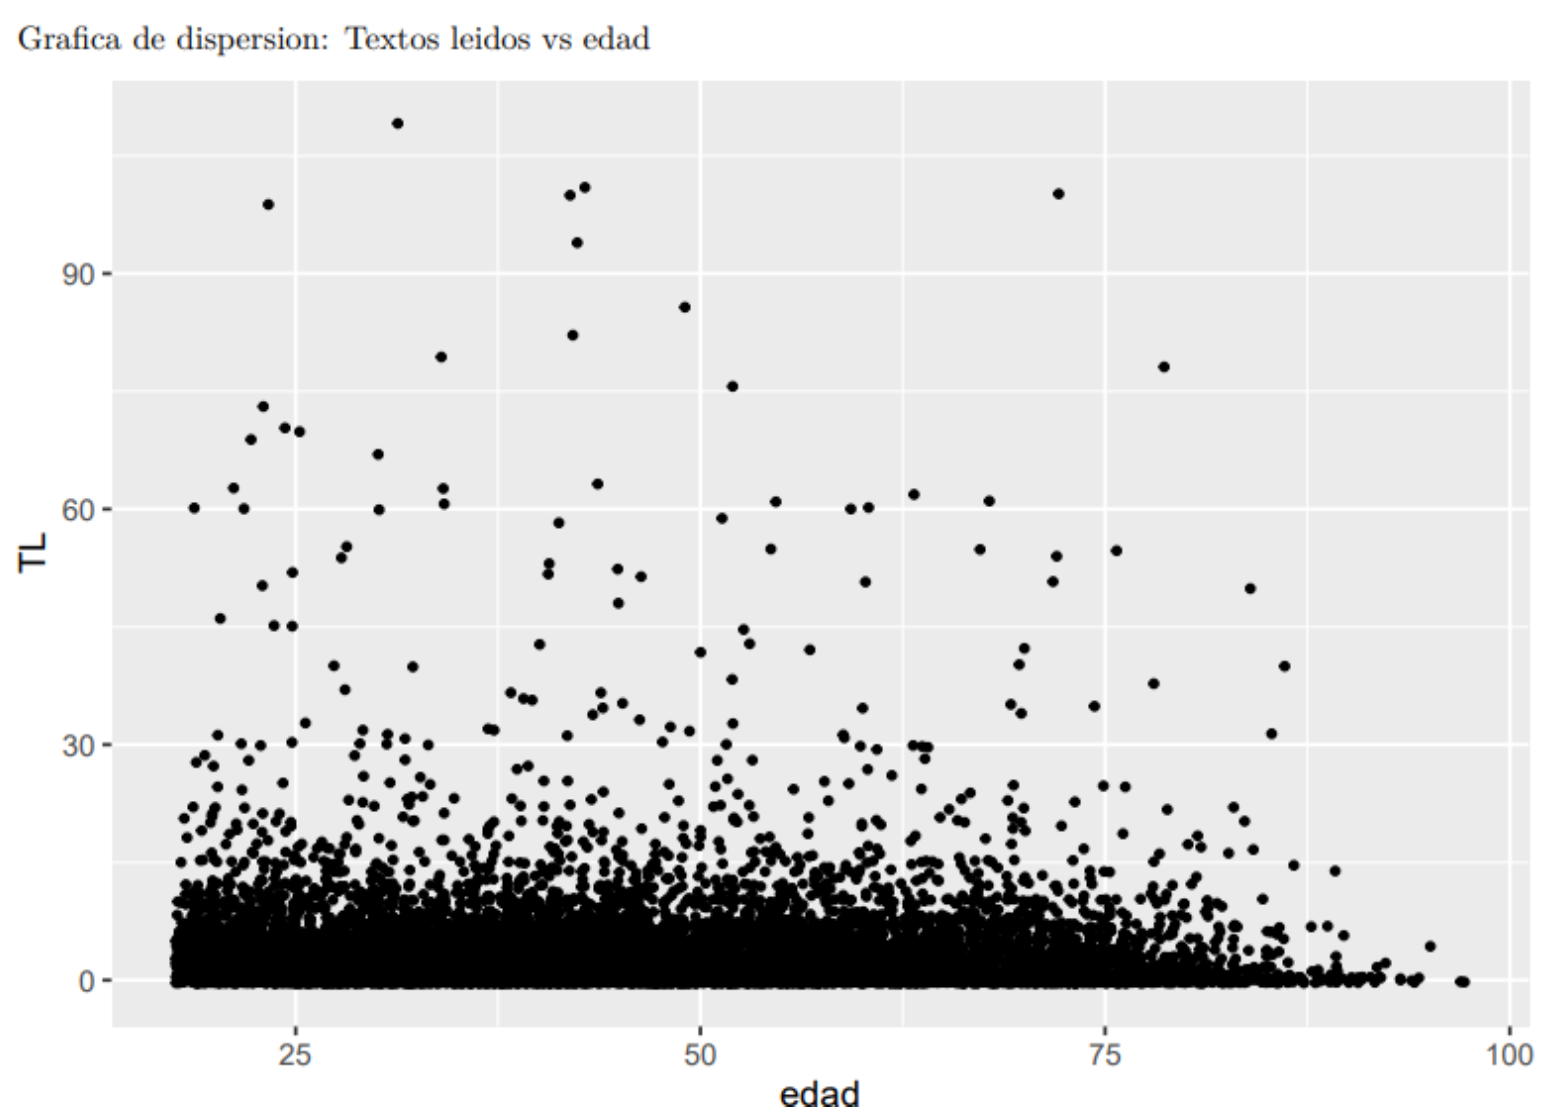
\includegraphics[width=0.4\textwidth]{Screenshot 2025-10-10 at 15.16.28.png}
    \caption{Grafico de dispersion de textos leidos contra edad}
    \label{fig:grafico_dispersion}
\end{figure}

Esta es una gráfica de dispersión donde en el eje x se encuentra la variable de la edad,
mientras que en el eje y se encuentra la cantidad de textos leídos como variable. De esta
gráfica lo que podemos observar es que la mayoría del valor se encuentra concentrada en
valores menores a 15, además de que, si prestamos atención, realmente los datos están
distribuidos de una manera muy uniforme a lo largo de toda la gráfica a excepción de cuando
las personas tienen más de 70 años, donde aquí es donde se comienza a observar como
empieza a reducirse la cantidad de textos leídos, lo cual tiene sentido por motivos de salud
que lean menos. Además, en la gráfica se puede notar como es que hay una gran cantidad de
valores atípicos, lo cual, junto con constante cerca de 0, hace aún más difícil el poder
encontrar una correlación entre la edad y la cantidad de textos leídos o en el hábito de la
lectura.

\begin{figure}[H]
    \centering
    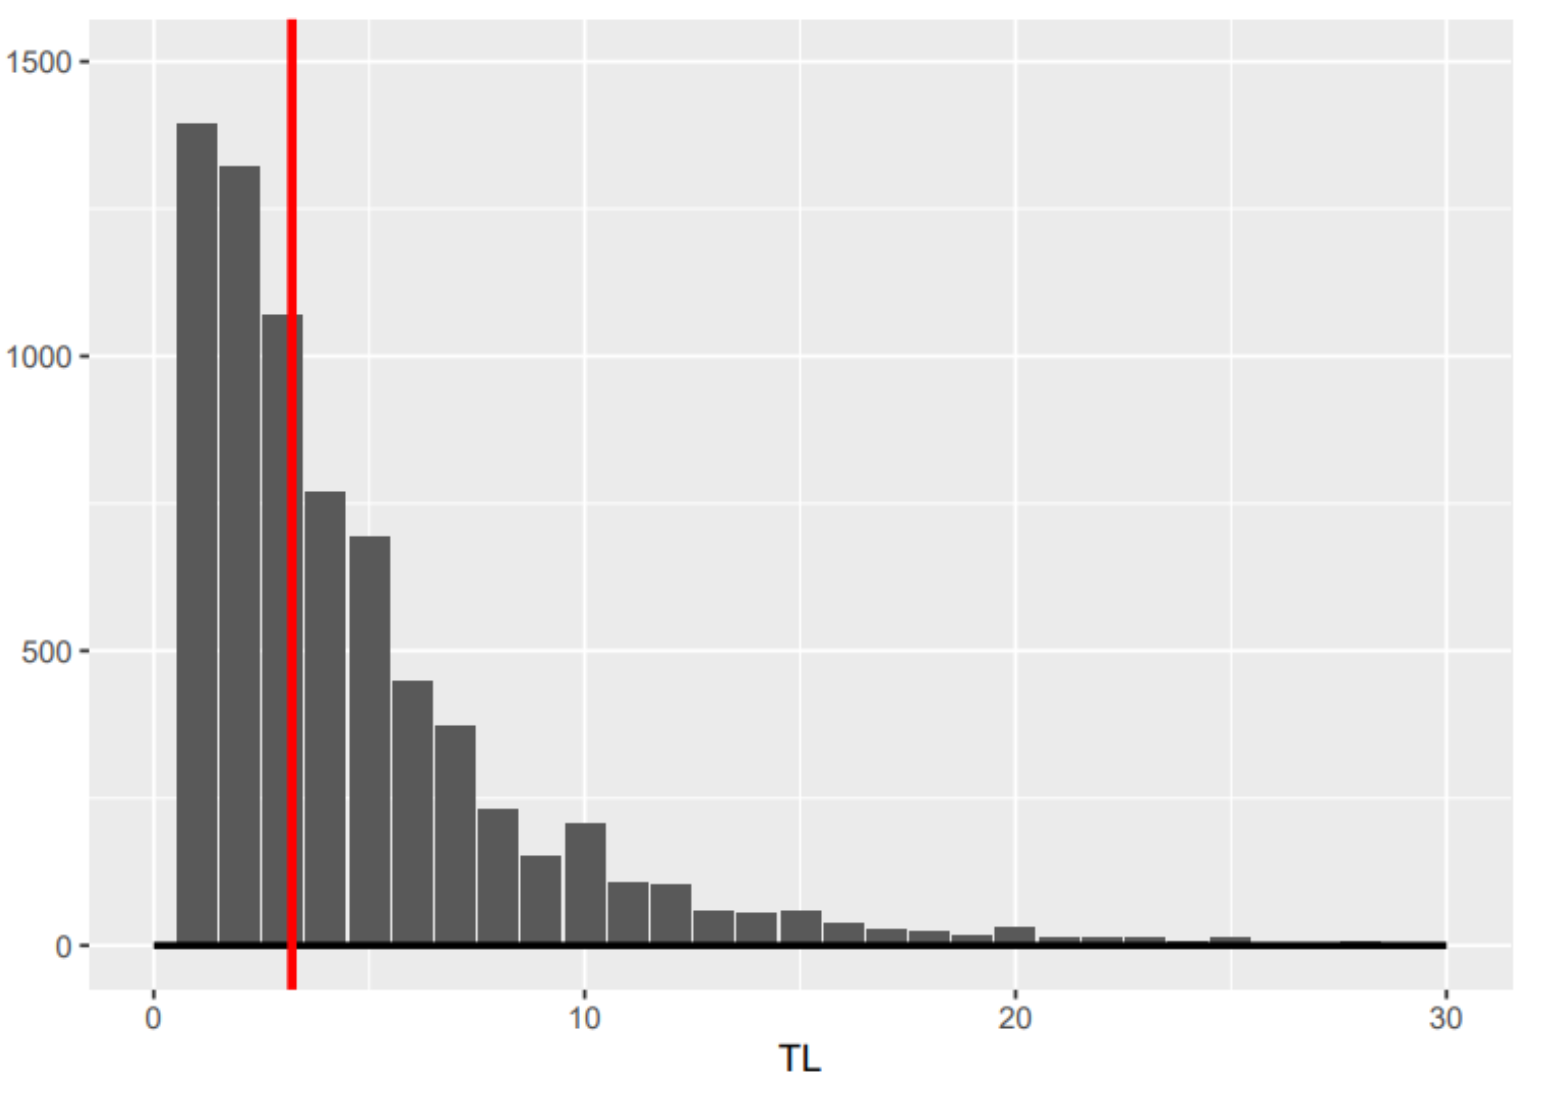
\includegraphics[width=0.4\textwidth]{Screenshot 2025-10-10 at 15.17.58.png}
    \caption{Histograma}
    \label{fig:hist}
    
\end{figure}

En este histograma, en el eje de las x se encuentra como variable la cantidad de textos leídos,
mientras que en el eje de las y el número de personas que han leída tal cantidad de libros. Se
puede notar como el histograma tiene un gran sesgo positivo, lo cual significa que la mayoría
de las personas han leído una muy pequeña cantidad de textos y conforme la cantidad de
textos leídos va aumentando la cantidad de personas que cumplen con este requisito
disminuye exponencialmente. Gracias a la línea roja en el histograma, nos indica que en
promedio las personas han leído aproximadamente 3 textos, lo cual simboliza una gran área
de oportunidad en el ámbito de la lectura.

\begin{figure}[H]
    \centering
    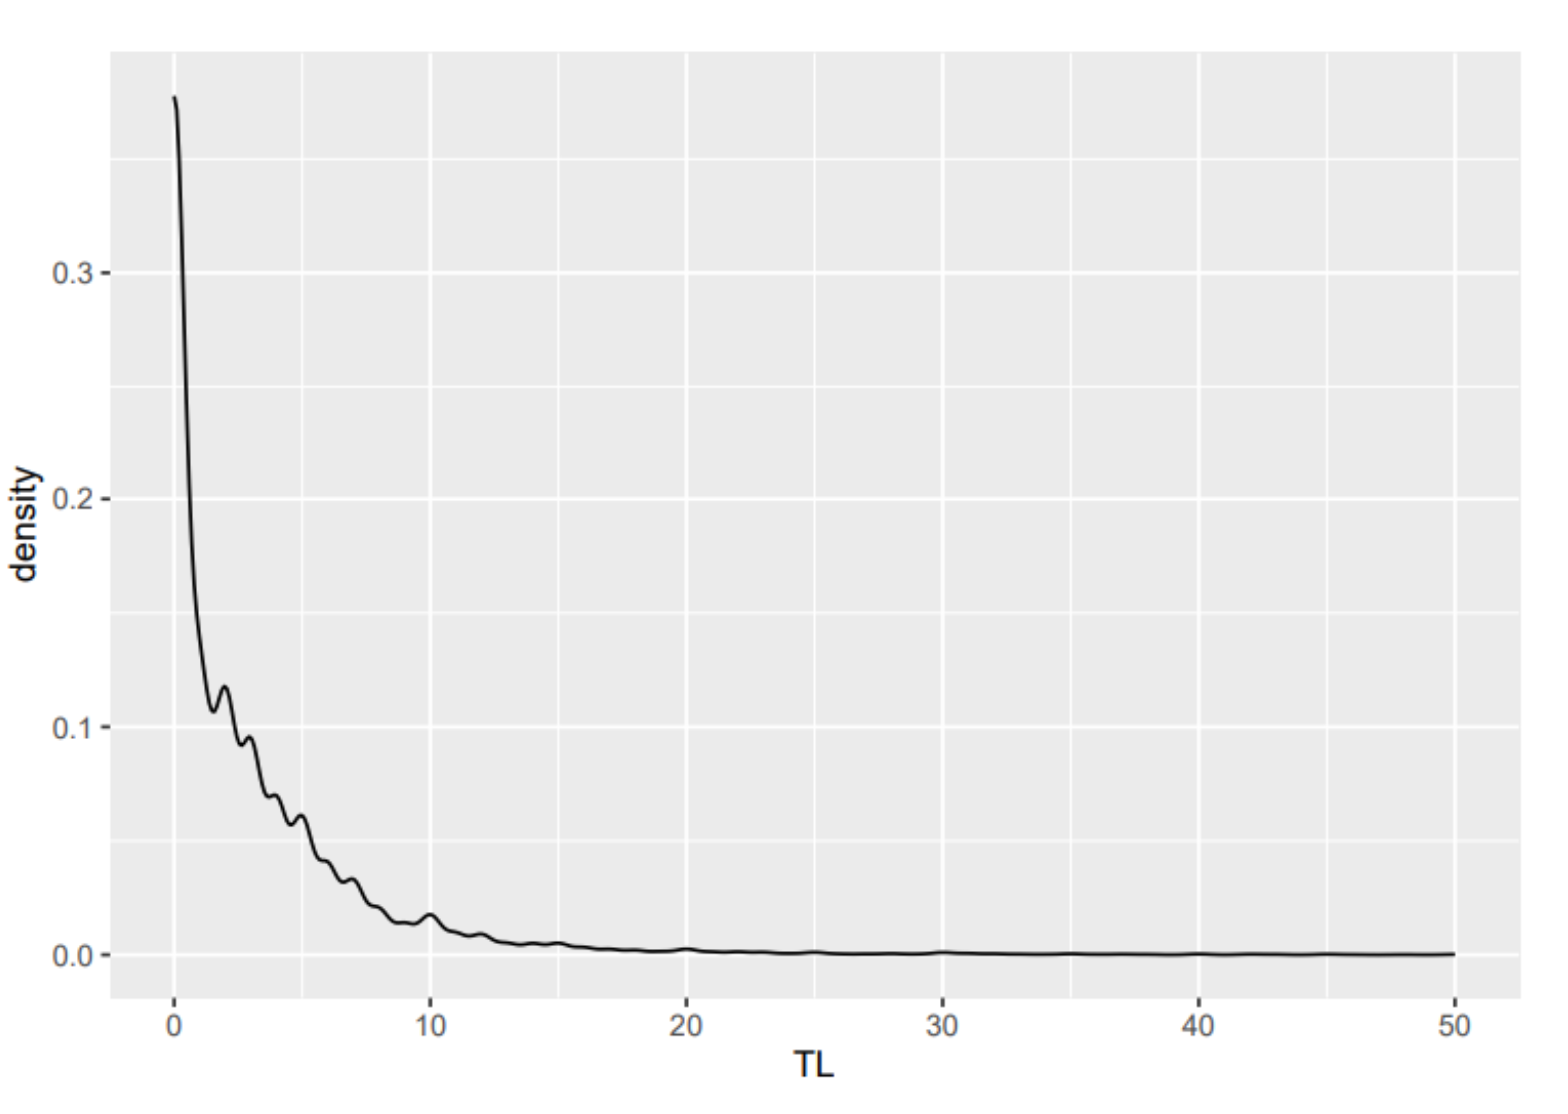
\includegraphics[width=0.4\textwidth]{Screenshot 2025-10-10 at 15.19.29.png}
    \caption{Grafico de densidad}
    \label{fig:densidad}
    
\end{figure}

En esta gráfica se muestra en el eje x la cantidad de textos leído mientras que en el eje y el
porcentaje de personas que corresponden a dicho valor. Como se puede observar por el sesgo
alto sesgo a la derecha o positivo, el mayor porcentaje se encuentra del lado izquierdo o
donde hay menos libros leídos, habiendo poco menos del 40\% con 0 textos leídos y
decreciendo exponencialmente según aumenta la cantidad de textos leídos, siendo ya 6 textos
leídos significando menos del 5\% de la población.

\begin{figure}[H]
    \centering
    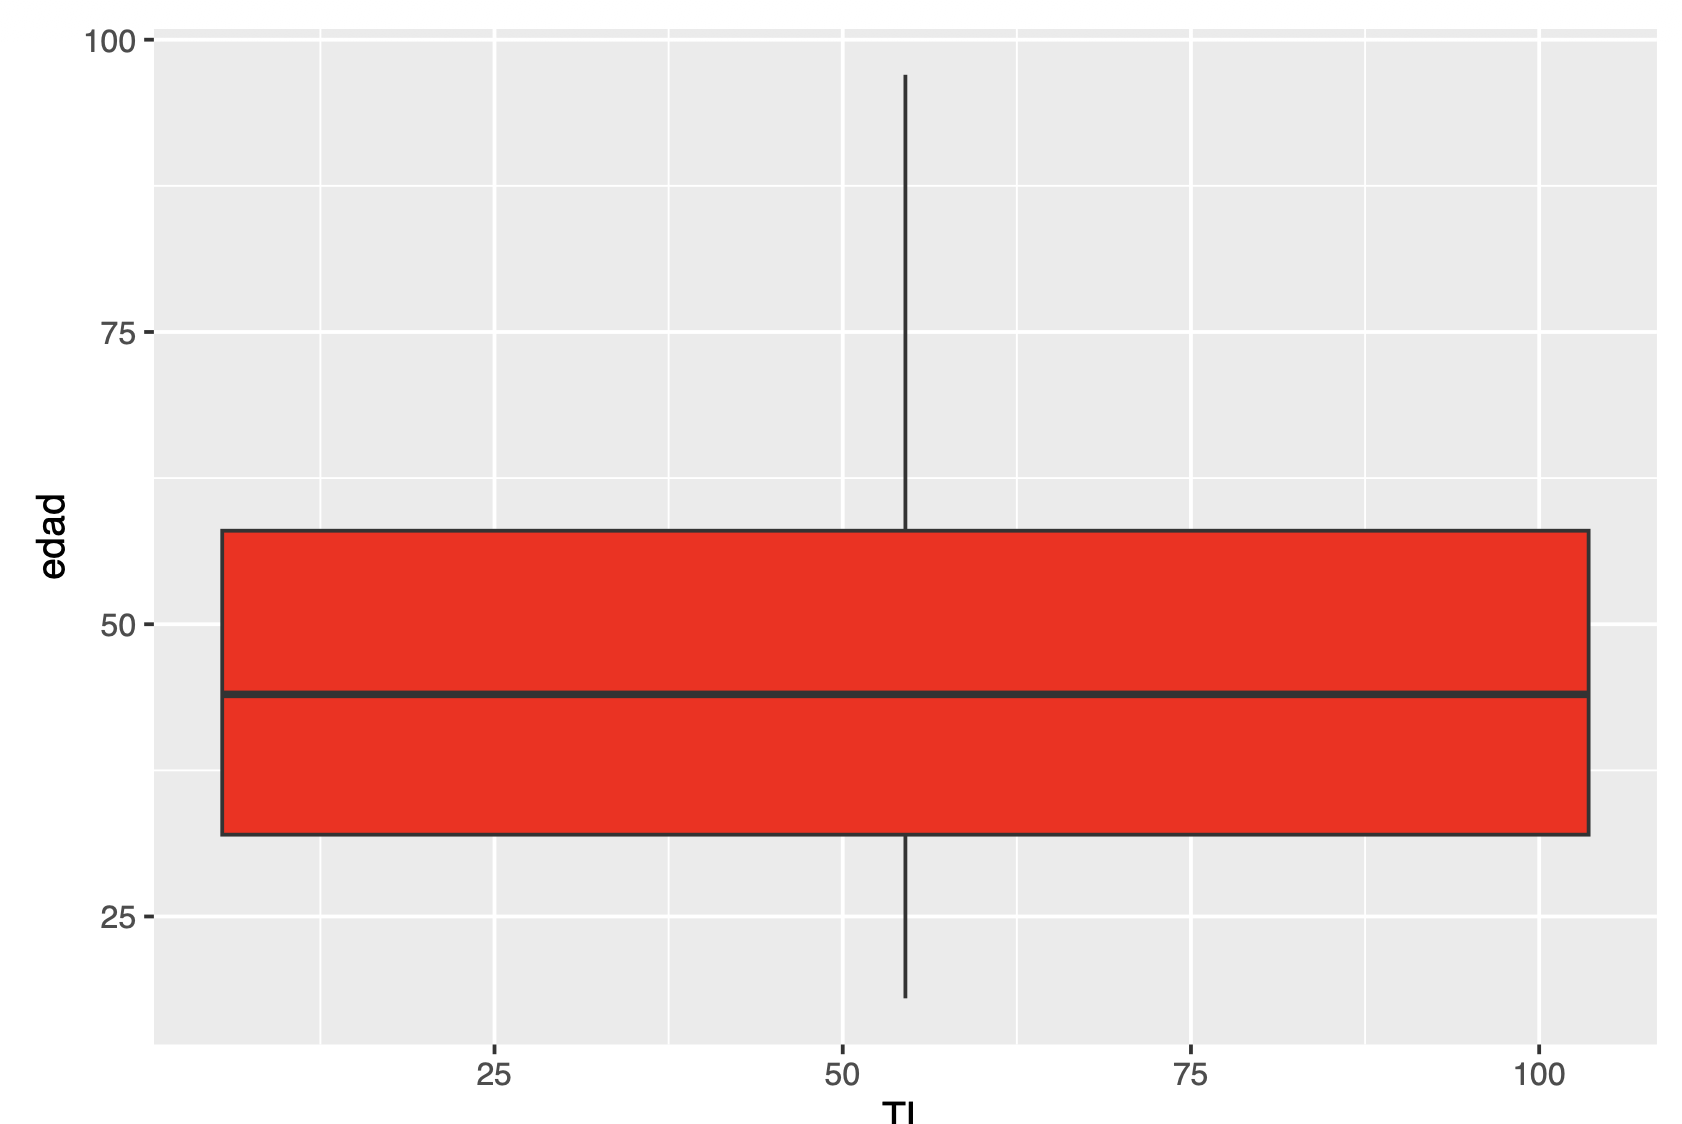
\includegraphics[width=0.4\textwidth]{Screenshot 2025-10-10 at 15.21.24.png}
    \caption{Grafico de caja}
    \label{fig:caja}
    
\end{figure}

En este boxplot podemos observar como están distribuidos los datos siendo el eje x cantidad
de textos leídos y el eje y edad. En este boxplot podemos ver como por la media en promedio
las personas que más leen están alrededor de 42 años, además de que se encuentran entre las
edades un poco más altas, como de 30 a 60 años, por lo cual se podría intuir que esto provenga
por crianzas o infancias diferentes o incluso que simplemente sea un hábito que se va
desarrollando más con la madurez.

\begin{figure}[H]
    \centering
    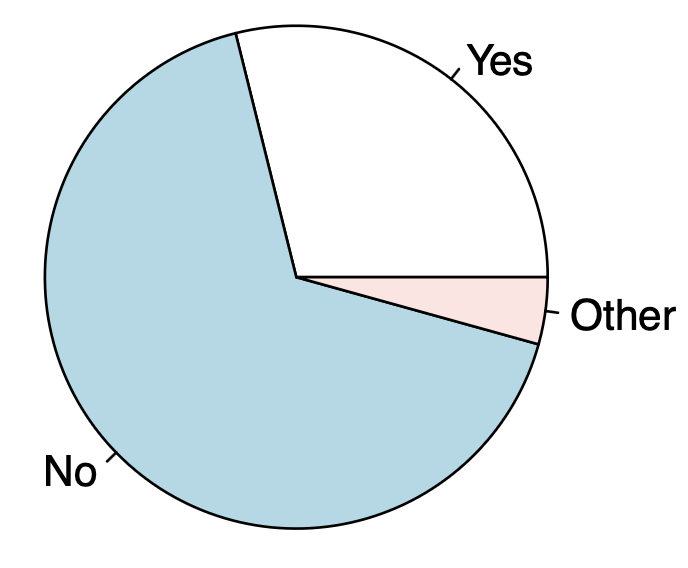
\includegraphics[width=0.4\textwidth]{Screenshot 2025-10-10 at 15.23.46.png}
    \caption{}
    \label{fig:pie}
    
\end{figure}

En la anterior gráfica de pastel el área azul representa el porcentaje de personas que no fueron
llevados a la biblioteca en la infancia, mientras que el área negra representa el porcentaje que
si y por otro lado el área roja personas que saltaron la pregunta. En esta gráfica podemos
observar como la cantidad de personas que fueron llevadas a bibliotecas o librerías en la
infancia representa poco más de un cuarto de la población, lo cual representa muy poco
porcentaje y podría ser un indicio por el cuál de adultos la cantidad de textos que leen las
personas es muy baja.

\begin{figure}[H]
    \centering
    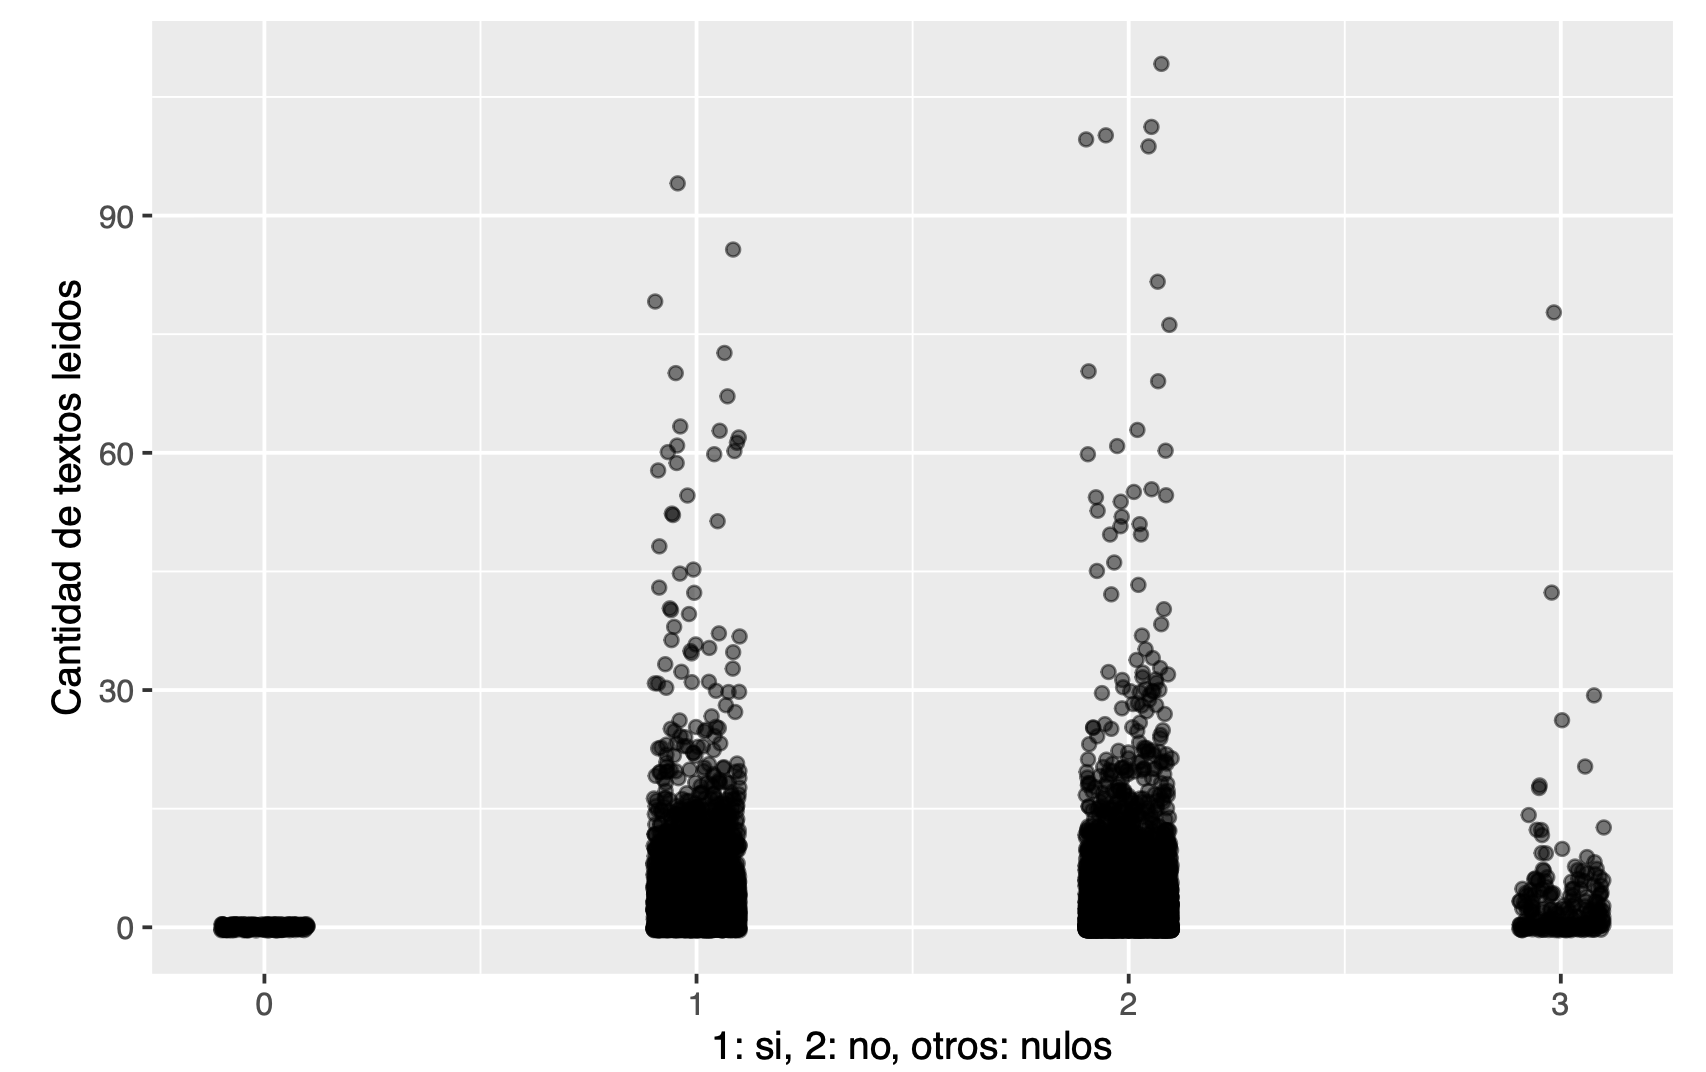
\includegraphics[width=0.4\textwidth]{Screenshot 2025-10-10 at 15.25.33.png}
    \caption{Grafico de cantidad de textos leidos y si fueron a librerias en su infancia}
    \label{fig:TL_LI}
    
\end{figure}

En esta gráfica se encuentra en el eje de las x las personas que en la infancia fueron llevadas
a una biblioteca o a una librería, siendo el numero 1 las personas que, si fueron llevadas a
uno de estos lugares, siendo el numero 2 personas que no fueron llevadas y siendo el numero
3 personas que se saltaron la pregunta, mientras que en el eje de las y, podemos observar la
cantidad de libros que leyeron cada persona. Como se puede observar en la gráfica, las
personas que fueron llevadas en la infancia a una biblioteca y las que no, tienen una cantidad
de libros muy similar, ya que en ambos casos se encuentra sobre todo la mayor cantidad de
personas habiendo leído menos de 15 textos, donde a partir de ese número decrece en gran
medida en ambos casos, habiendo outlyers en los dos casos. Es por eso por lo que no se puede
afirmar con seguridad que el hecho de en la infancia hayan sido llevados a bibliotecas o
librerías tenga un impacto significativo en la cantidad de libros leídos en la edad adulta.

\begin{figure}[H]
    \centering
    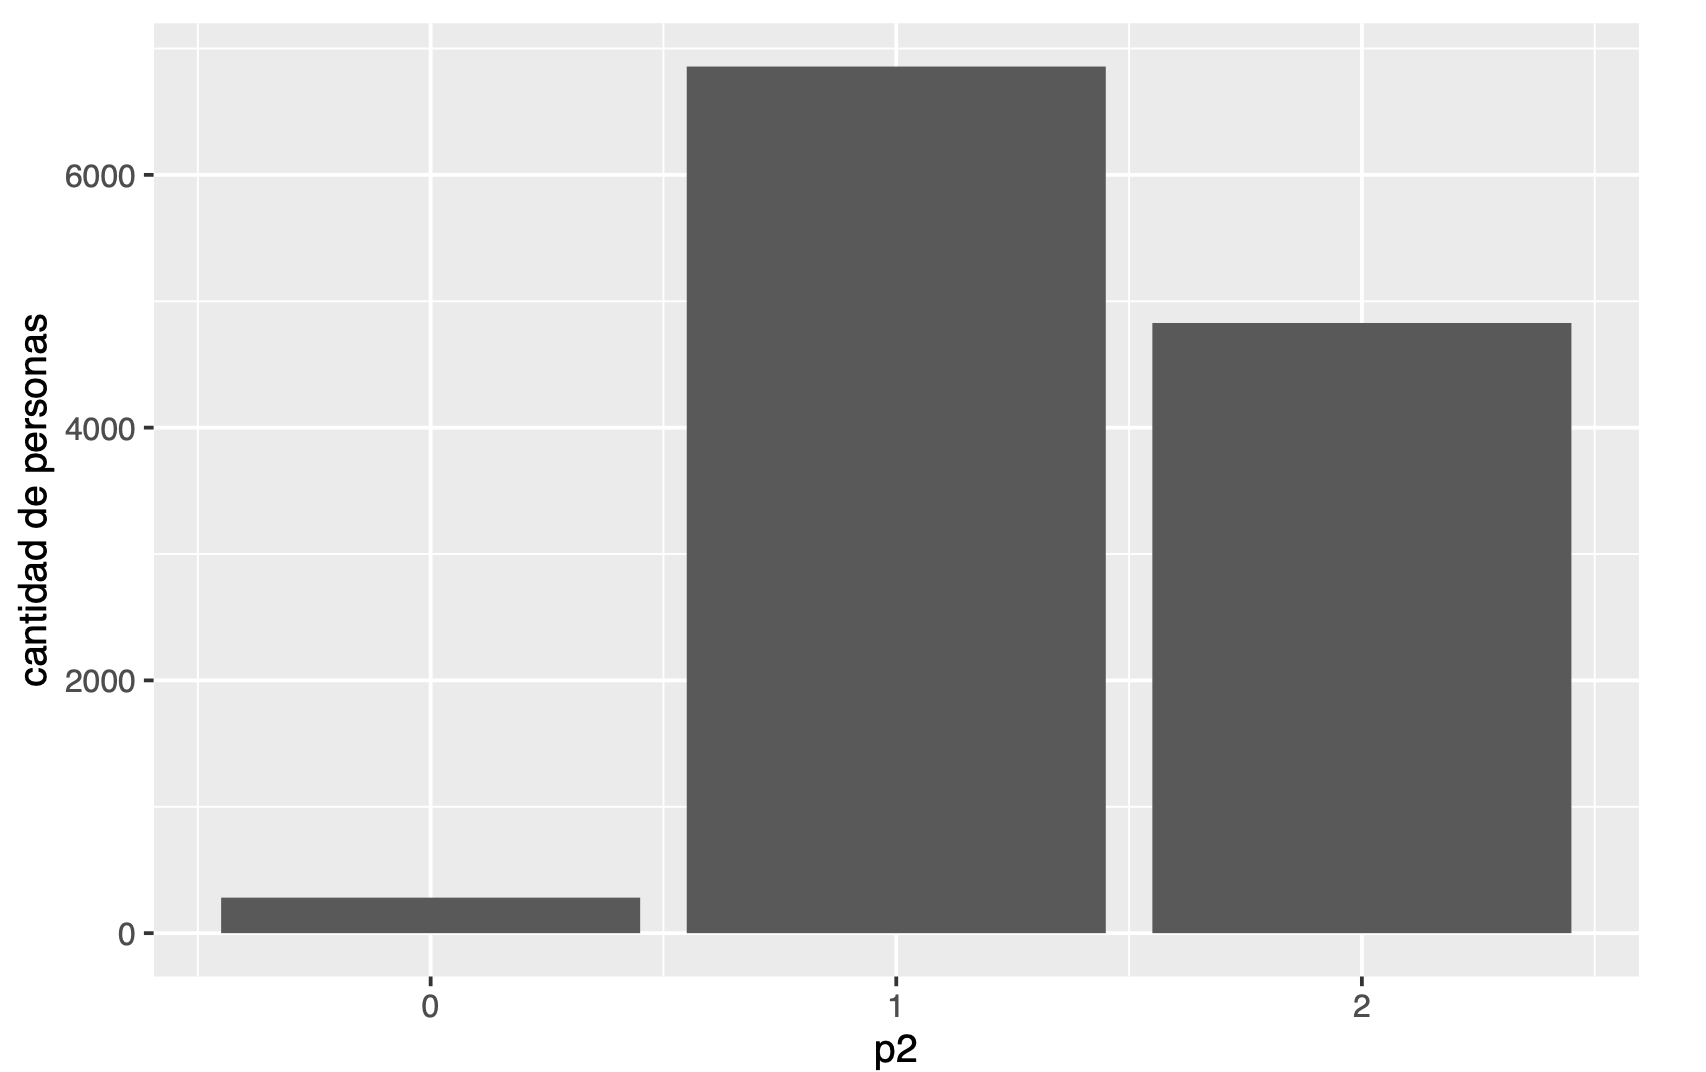
\includegraphics[width=0.4\textwidth]{Screenshot 2025-10-10 at 15.28.33.png}
    \caption{Grafico de barras, repuesta a la pregunta ¿Acostumbra leer?}
    \label{fig:leer_acostumbra}
    
\end{figure}

Finalmente, en este gráfico en el eje x se encuentra con el valor de 1 las personas que
acostumbran a leer mientras que con el número 2 las personas que no acostumbran a leer,
siendo el eje y la cantidad de personas dieron esa respuesta. Por lo que podemos notar que la
mayoría de las personas que contestaron la encuesta sí acostumbra a leer, siendo las personas
que no acostumbran a hacerlo poco más de 2/3 de los que sí lo acostumbran.

\subsubsection{Conclusiones del análisis descriptivo}


Este análisis nos permitió tener una primera aproximación a la pregunta inicial: si el estímulo de lectura durante la infancia influye en el desarrollo del hábito lector en la edad adulta. Los resultados muestran que las experiencias familiares a temprana edad se asocian con una mayor probabilidad de que las personas lean de grandes.

Hasta el momento, hemos logrado identificar las variables más relevantes, detectar datos faltantes, encontrar errores y limpiar la base de datos. Se realizó una descripción del comportamiento que tienen las variables demográficas, de estímulo y de resultados.

Fue importante encontrar patrones iniciales que sugieren una relación positiva entre los estímulos de lectura a temprana edad y el hábito de leer en una etapa adulta.

Nos falta realizar un análisis inferencial en el cual confirmemos estadísticamente si todas las relaciones son significativas, utilizando las variables planteadas, como la edad, el sexo y el nivel educativo.

También es necesario hacer un mayor énfasis en las diferencias de regiones y de género en los hábitos de lectura, además de explorar modelos que permitan cuantificar la influencia de los estímulos en la probabilidad de tener un mayor porcentaje de lectura en la edad adulta.

El siguiente paso será aplicar pruebas de independencia y análisis de correlación entre las variables de estímulo y las variables del hábito de lectura, con el fin de plantear un modelo que nos permita validar nuestra hipótesis central.

Durante el desarrollo nos surgieron preguntas como:
\begin{itemize}
    \item ¿Cuál es el estímulo que tiene mayor peso en el hábito de la lectura?
    \item ¿La diferencia entre regiones en el efecto de promover la lectura es muy grande?
    \item ¿La influencia del entorno familiar podría superar al impacto que tiene la educación sobre este hábito?
\end{itemize}

Nuestro análisis descriptivo confirma que el entorno familiar sí es un componente esencial en la formación del hábito lector, y constituye la base principal para avanzar en el análisis y continuar con la siguiente etapa del proyecto.

\section{Análisis inferencial}
\subsection{Objetivo del análisis}

El objetivo que planteamos desde el principio para nuestro proyecto se mantiene igual al que establecimos en la Etapa 1, ya que seguimos enfocados en evaluar si los estímulos lectores que se presentaron durante la infancia impactan en el desarrollo del hábito de la lectura en la edad adulta. No realizamos modificaciones al objetivo original, ya que continúa siendo adecuado para responder a la pregunta de investigación.

\subsection{Análisis inferencial: Hipótesis e intervalos de confianza}

El análisis inferencial permitió comprobar si la exposición adecuada a los estímulos de lectura durante la infancia determina los hábitos lectores en la adultez. Para ello, se emplearon diferentes técnicas estadísticas como las \textbf{pruebas de hipótesis} y los \textbf{intervalos de confianza}.

\subsubsection*{Técnicas estadísticas utilizadas}
Las pruebas de hipótesis permiten determinar si existen diferencias o relaciones estadísticamente significativas entre grupos o variables, mientras que los intervalos de confianza estiman rangos de posibles valores para proporciones, medias y varianzas. Estos métodos permiten evaluar la precisión de los estimadores de muestra asociados al comportamiento lector.

\subsubsection*{Resultados de las pruebas de hipótesis}

\paragraph{Prueba 1: Influencia de haber visto leer a los padres}
\begin{itemize}
    \item \textbf{Hipótesis nula (H$_0$):} No hay relación entre haber visto leer a los padres (P34\_2) y leer por gusto en la adultez (P5 = 4).
    \item \textbf{Hipótesis alternativa (H$_1$):} Existe relación entre ambas variables.
    \item \textbf{Resultado:} Se rechazó la hipótesis nula.
\end{itemize}
Esto indica que observar a los padres leer durante la infancia incrementa la probabilidad de desarrollar gusto por la lectura en la adultez. En relación con el objetivo, este resultado apoya la idea de que los modelos familiares de lectura influyen en el hábito lector posterior.

\paragraph{Prueba 2: Libros en casa durante la infancia}
\begin{itemize}
    \item \textbf{Hipótesis nula (H$_0$):} La media de libros leídos por quienes tuvieron libros en casa es igual a la de quienes no los tuvieron.
    \item \textbf{Hipótesis alternativa (H$_1$):} Las personas que crecieron con libros en casa leen más libros.
    \item \textbf{Resultado:} Se rechazó la hipótesis nula.
\end{itemize}
Esto demuestra que haber tenido acceso a libros en casa tiene un efecto positivo y duradero sobre la actividad lectora en la edad adulta.

\paragraph{Prueba 3: Diferencias por sexo}
\begin{itemize}
    \item \textbf{Hipótesis nula (H$_0$):} No existen diferencias en la media de textos leídos entre hombres y mujeres.
    \item \textbf{Hipótesis alternativa (H$_1$):} Las mujeres leen más textos que los hombres.
    \item \textbf{Resultado:} No se rechazó la hipótesis nula.
\end{itemize}
No se observaron diferencias significativas entre hombres y mujeres en la cantidad de textos leídos, lo cual sugiere que las diferencias lectoras no dependen del sexo, sino de experiencias lectoras durante la infancia.

\paragraph{Prueba 4: Asistencia a bibliotecas o librerías durante la infancia}
\begin{itemize}
    \item \textbf{Hipótesis nula (H$_0$):} No hay relación entre haber asistido a bibliotecas/librerías (P34\_1) y el hábito lector actual (P2).
    \item \textbf{Hipótesis alternativa (H$_1$):} Sí existe relación entre ambas variables.
    \item \textbf{Resultado:} Se rechazó la hipótesis nula.
\end{itemize}
Este hallazgo evidencia que haber visitado espacios de lectura en la infancia incrementa la probabilidad de ser lector en la adultez, reforzando el papel de las experiencias formativas fuera del hogar en el desarrollo del interés lector.

\subsubsection*{Resultados de los intervalos de confianza}

\paragraph{1. Proporción de personas que leen por gusto (P5 = “Gusto/Entretenimiento”)}
\begin{itemize}
    \item \textbf{Punto de estimación:} $p = 0.4232$
    \item \textbf{IC (96\%):} [0.4086, 0.4377]
\end{itemize}
Se puede afirmar con un 96\% de confianza que entre el 40.9\% y el 43.8\% de las personas leen por gusto. Esta proporción relativamente baja sugiere que la lectura por placer no es la principal motivación, siendo más frecuentes motivos académicos o escolares. Esto destaca la necesidad de estrategias de fomento lector más intensivas.

\paragraph{2. Diferencia de proporciones según tener libros en casa}
\begin{itemize}
    \item \textbf{Estimación puntual:} $p_1 - p_2 = 0.0109$
    \item \textbf{IC (96\%):} [$-0.0229$, $0.0446$]
\end{itemize}
Como el intervalo incluye el cero, no se puede afirmar que la diferencia sea significativa. Sin embargo, la ligera diferencia positiva refuerza la tendencia observada: quienes tuvieron libros en casa tienden a leer más, aunque el efecto en proporciones es pequeño.

\paragraph{3. Media del total de textos leídos (TL)}
\begin{itemize}
    \item \textbf{Media:} 3.2057
    \item \textbf{Desviación estándar:} 6.028
    \item \textbf{IC (96\%):} [3.0925, 3.3189]
\end{itemize}
El promedio de textos leídos anualmente se sitúa entre 3 y 3.3 materiales. Esto indica una baja intensidad lectora general, sugiriendo que los estímulos tempranos influyen más en la \emph{frecuencia} de lectura que en el número total de materiales.

\paragraph{4. Varianza en libros leídos (P4)}
\begin{itemize}
    \item \textbf{Varianza de la muestra:} 14.84
    \item \textbf{IC (96\%):} [14.46, 15.24]
\end{itemize}
La estrechez del intervalo refleja una estimación precisa y evidencia una alta dispersión en los hábitos lectores: existen personas que leen mucho y otras que apenas leen.

\vspace{-0.8em}
\subsection{Conclusión del análisis inferencial}

El análisis inferencial nos permitió confirmar con evidencias estadísticas que en la infancia los niños que están rodeados de estímulos lectores presentan un desarrollo positivo en el hábito de la lectura a una edad adulta. Comprobamos que si eran llevados a bibliotecas, observaban a sus padres leer o contaban con libros en casa, son factores que incrementan la probabilidad en etapas posteriores. También identificamos que la variable del sexo no presenta grandes diferencias en la cantidad de lectura de las personas, pero sí hay cierta diferencia entre regiones y niveles educativos, esto nos indica que las desigualdades sociales y el acceso a materiales sí tienen un impacto en este hábito.

Nuestros principales logros fueron realizar la limpieza de datos, realizar una validación completa a la base de datos, además de describir las variables que utilizamos y explorar variables cuantitativas y cualitativas. La aplicación de pruebas de hipótesis e intervalos de confianza refuerzan nuestras conclusiones. Proponemos como siguiente paso en nuestro proyecto realizar modelos predictivos que nos ayuden a obtener el peso de cada estímulo durante la infancia en la frecuencia de lectura adulta, y analizar la influencia utilizando factores culturales y educativos.

Con este análisis nos surgen preguntas como: ¿Cuál es el estímulo que tiene mayor influencia en la formación de la lectura? ¿La educación puede compensar que no se hayan tenido estímulos en la infancia?

\nocite{*}
\bibliographystyle{acm}
\bibliography{report_references.bib}
\end{document}